\documentclass[UTF8,oneside,cs4side]{ctexart}
\usepackage{xeCJK}
\usepackage{amsmath}
\usepackage{tabularx}
\usepackage{booktabs}
\usepackage{fancyhdr}
\usepackage{graphicx}
\usepackage{subcaption}
\pagestyle{fancy}
\fancyhf{}
\chead{描述统计学期末论文}
\cfoot{第\thepage 页}
\title{一元线性回归分析}
\author{钱昌发}
\date{2019年6月15日}
\begin{document}
	\maketitle
	\newpage
	改革开放以来,中国的经济得到飞速发展,人民的生活水准也得得到了极大的提高,中国的巨大进步的一个静待你例子就是在2016年宣布的全国的国内生产总值(GDP)已经超过日本,一时间这一消息瞬间传遍大江南北,一时间无论男女老少,无论是否知道国内生产总值这一概念,都开始传播中国已经``超越''日本,但是是否真的超越我们这里不讨论,但是可以看出的是,我国的经济水准得到了很大的提升,这一结论的证据就是国内生产总值的提升,知道并且了解国内生产总值的概念的人就无需多言,但常常有人问国内生产总值是不是我们自己和别人的所有的钱加一起的数量啊?回答当然是否定的,我给予的回答是和我们手里的钱有关,国内生产总值越大,就代表着我们自己越富,说完这些话的时候我自己就有点心虚,因为作为一个知识份子,说一些无根无据的话是很不好的,但是现在我就可以以我现在的知识来证明自己说的话。\par
	我这里使用居民消费水平来代表人们是否富裕,考虑到各省市生产总值存在较大差距,这里只选用一个省的地区生产总值,并用该地区居民消费水准来衡量富裕水准,登陆国家统计局整理安徽省近19年的数据得表\ref{tab1}\par
	利用MATLAB绘图得到关于表格数据得散点图,如图\ref{fig1}\par
	\begin{figure}[htb]
		\centering
		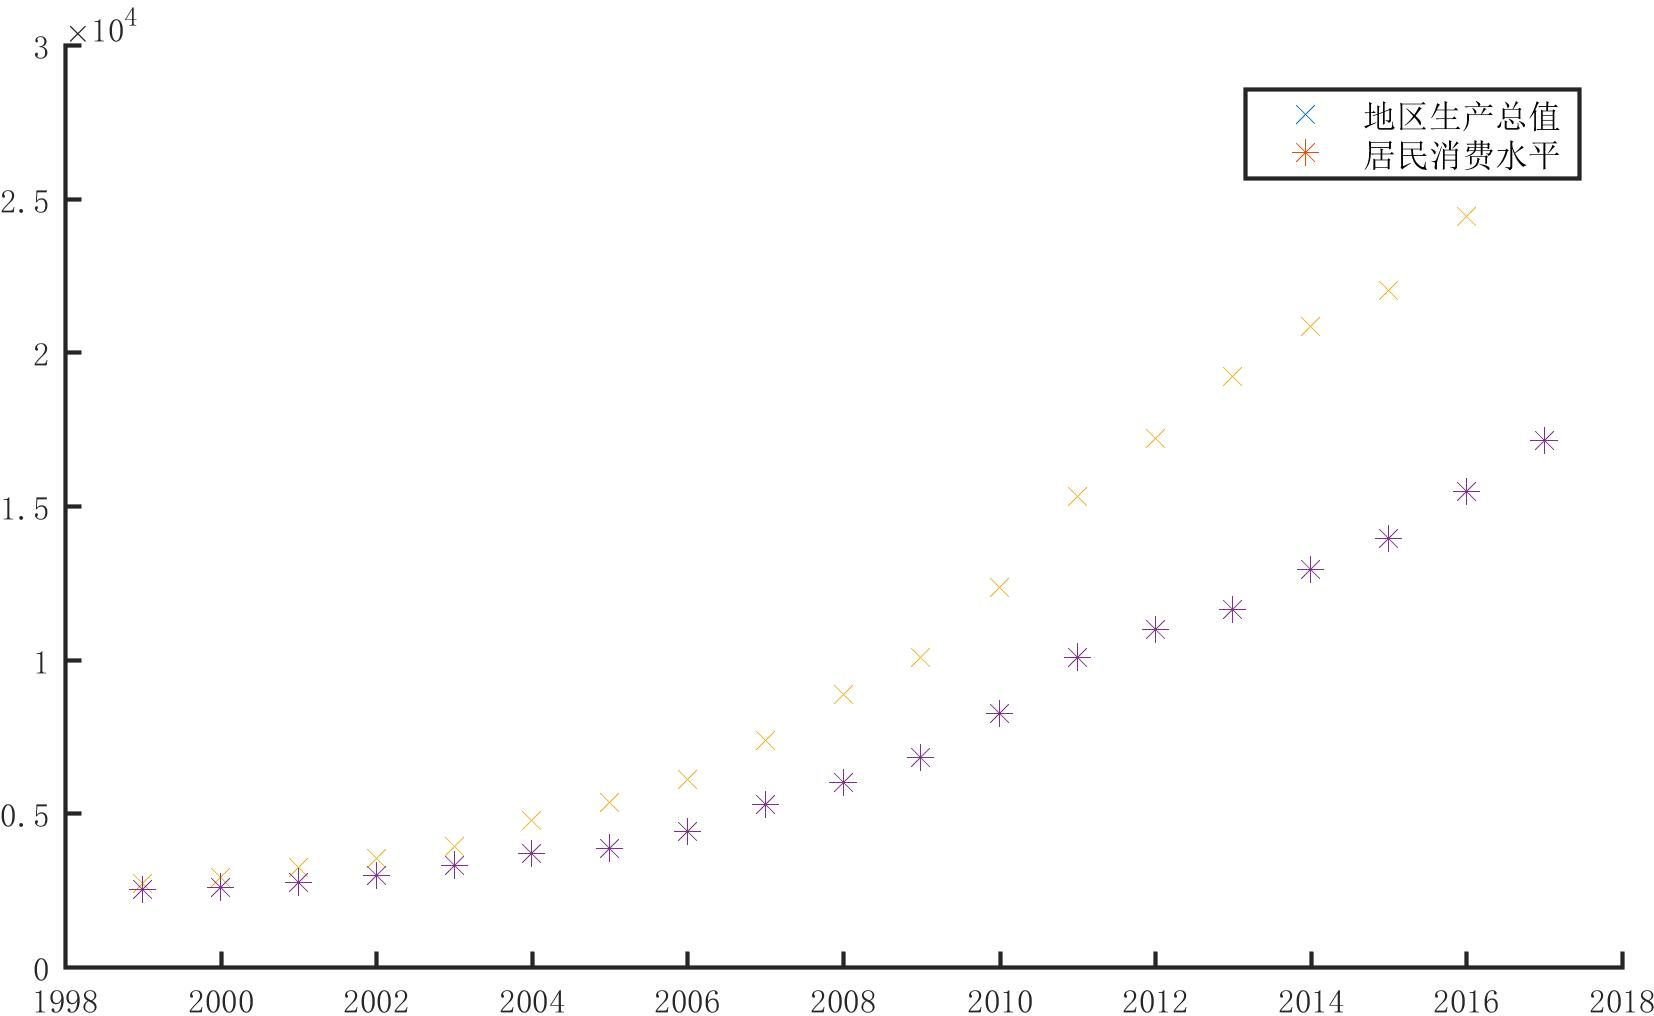
\includegraphics[width=0.9\textwidth]{fig1.jpg}
		\caption{关于年份的散点图}
		\label{fig1}
	\end{figure}
    可以看到居民消费水准与地区消费总值关于年份的散点图图形类似,可以猜测它们之间存在线性关系,所以画出居民消费水准关于地区消费总值的散点图,如图\ref{fig2}\par
    \begin{figure}[htb]
    	\centering
    	\begin{minipage}{1\textwidth}
    		\centering
    		\begin{subfigure}[b]{0.49\textwidth}\centering
    			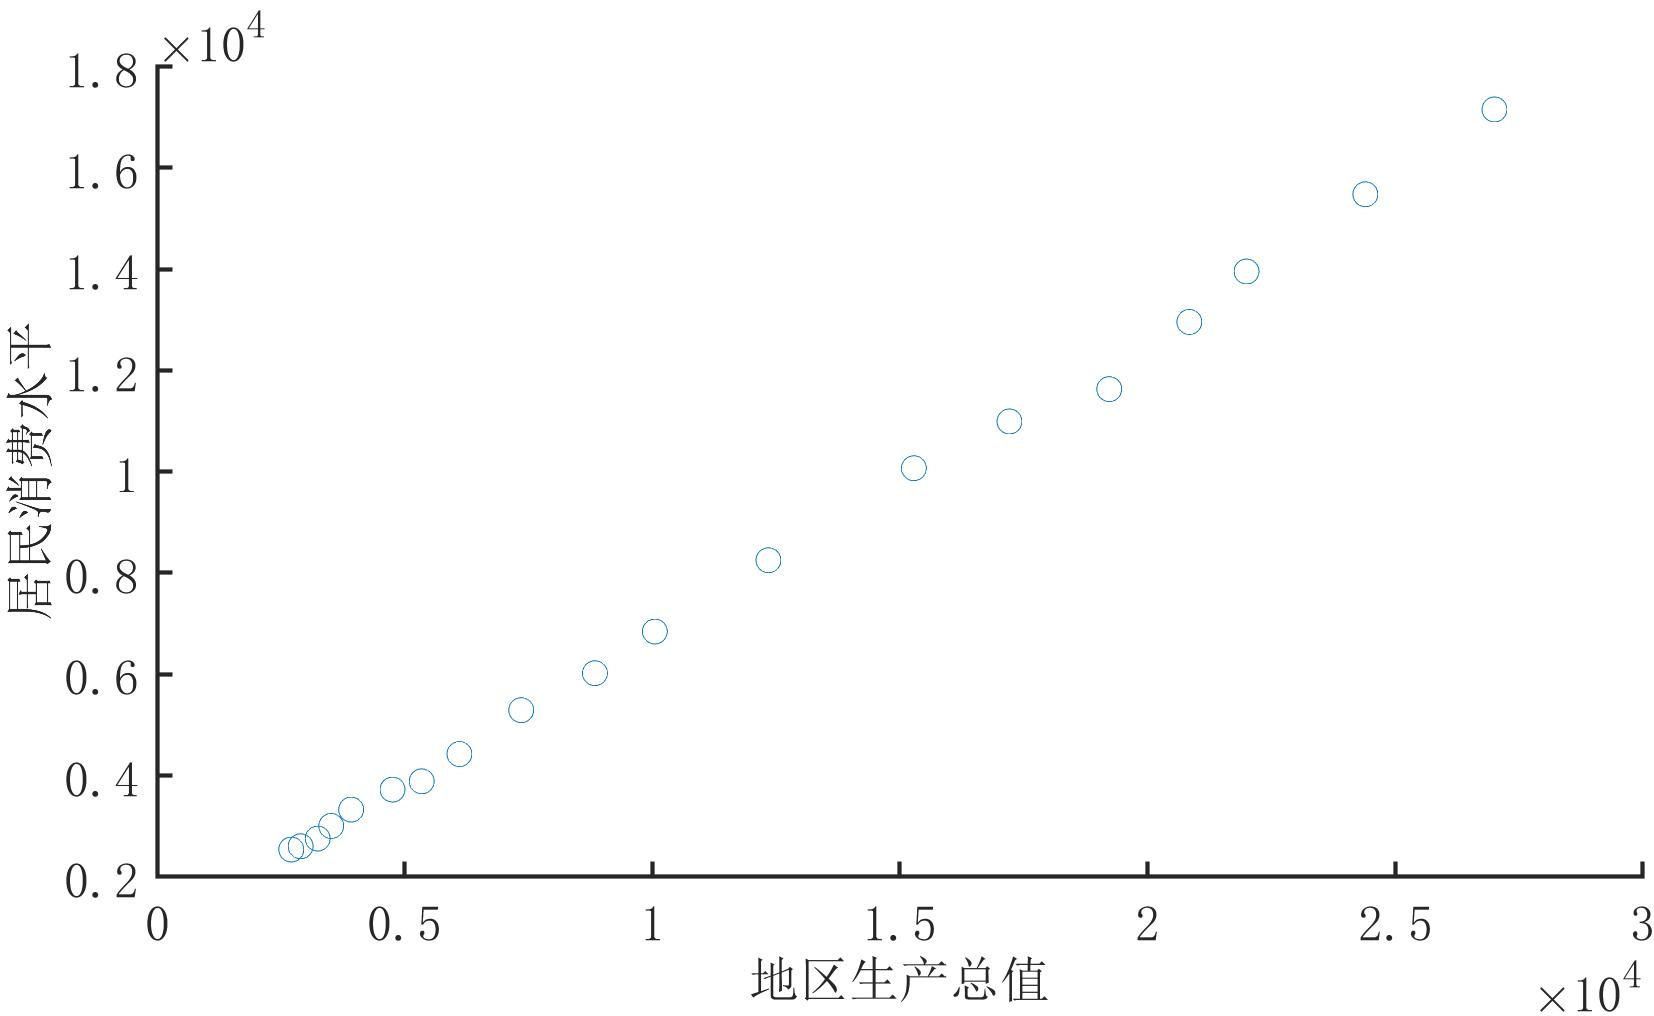
\includegraphics[width=0.9\textwidth]{fig2.jpg}
    			\caption{散点图}
    			\label{fig2}
    		\end{subfigure}
    		\begin{subfigure}[b]{0.49\textwidth}\centering
    			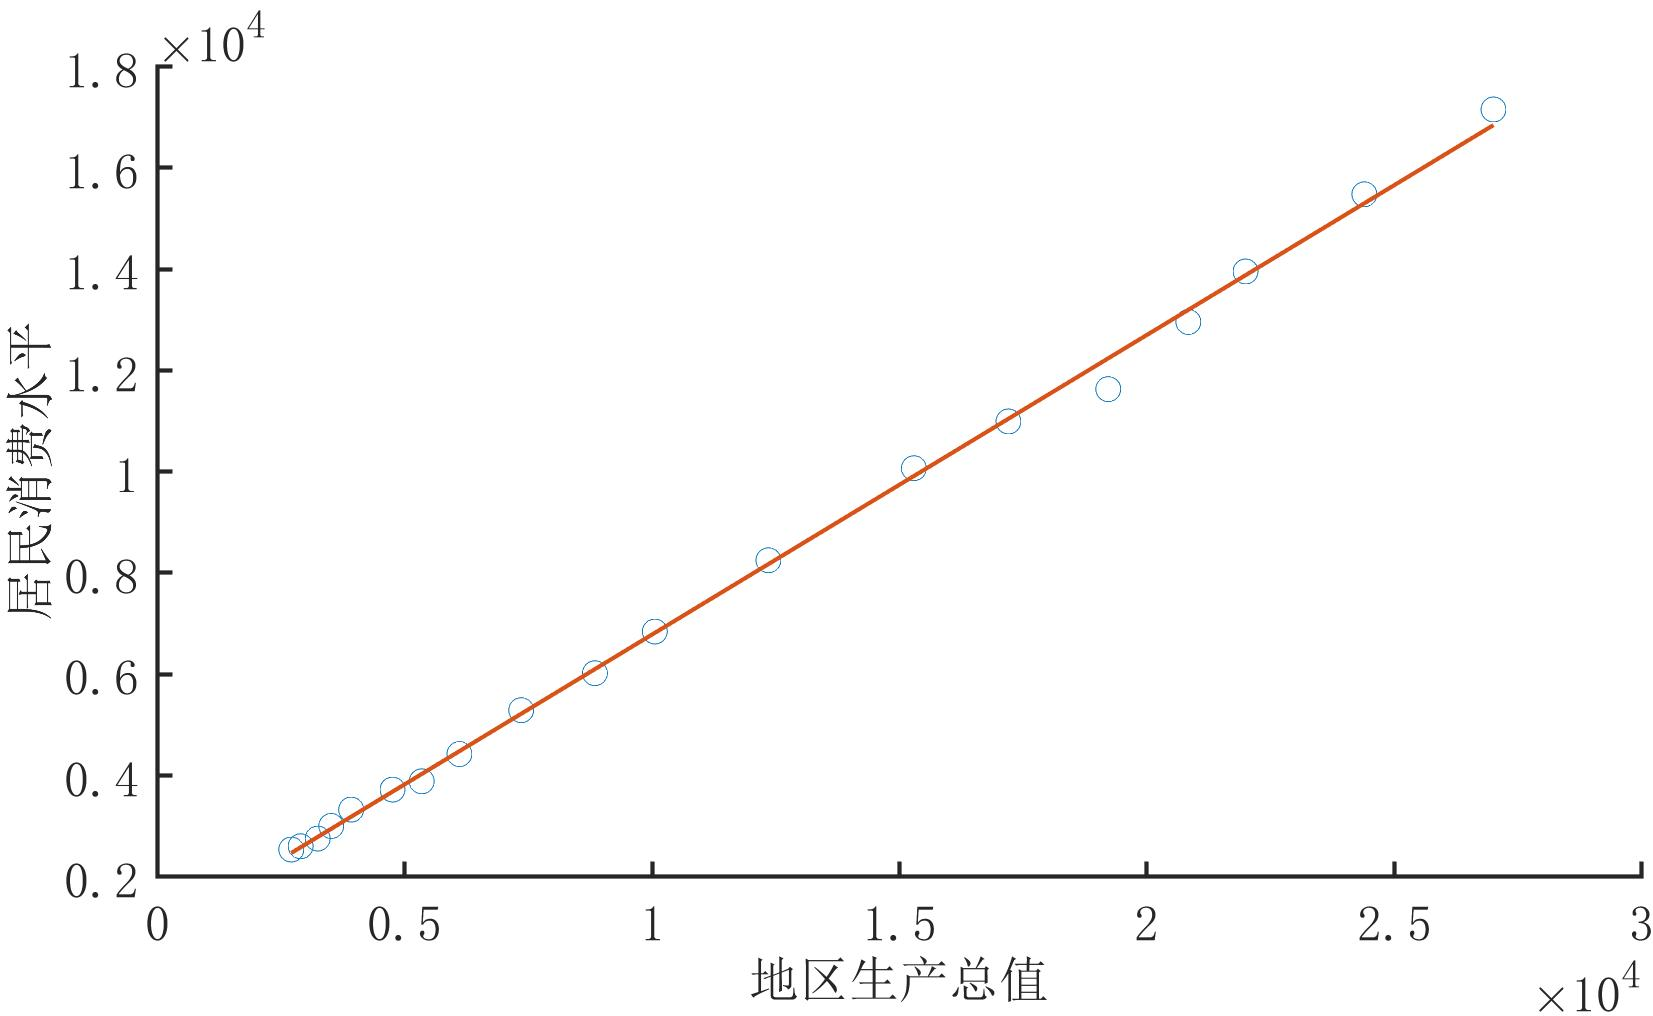
\includegraphics[width=0.9\textwidth]{fig3.jpg}
    			\caption{拟合曲线}
    			\label{fig3}
    		\end{subfigure}
    	\end{minipage}
    \end{figure}
    简单的观察图\ref{fig2},容易得出居民消费水准关于地区生产总值存在线性关系,以居民消费水平为因变量$Y$,以地区生产总值为$x$,建立一元线性回归模型:
    \begin{equation}
    Y=\beta_{0}+\beta_{1}x+\varepsilon
    \end{equation}
    其中$\varepsilon$为误差系数,是一个期望为零的随机变量,通过$n$个样本的值得到$\beta_{0},\beta_{1}$的估计值$\hat{\beta_{0}},\hat{\beta_{1}}$,得到样本回归函数:
    \begin{equation}
    \hat{y}=\hat{\beta_{0}}+\hat{\beta_{1}}x
    \end{equation}
    利用最小二乘法可以求得$\hat{\beta_{0}},\hat{\beta_{1}}$的值,这里利用MATLAB求解得到$\hat{\beta_{0}}=0.5916,\hat{\beta_{1}}=849.9176$,拟合曲线如图\ref{fig3}所示,这里可以看出拟合直线的拟合效果很好,可以通过Excel回归分析工具得到分析报告如图\ref{fig4}\par
    \begin{figure}[htb]
    	\centering
    	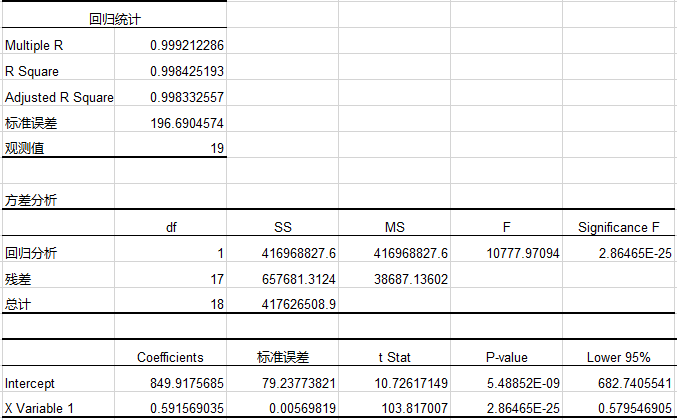
\includegraphics[width=0.9\textwidth]{fig4.png}
    	\caption{Excel回归分析结果}
    	\label{fig4}
    \end{figure}
    由图\ref{fig4}可以看出,$SSR=416968827.635,SSE=657681.312,SST=417626508.947,R_{2}=0.998425$,说明居民消费水平$y$由$99.8425\% $可以由$x$的变动来解释。\par
    现在对回归模型的显著性检验,即判断自变量$x$对因变量$y$是否由显著性影响,因此提出假设:
    \begin{equation}
    H_{0}:\beta_{1}=0 \longrightarrow H_{1}:\beta_{1}\not= 0
    \end{equation}
    对该假设进行检验将使用双尾$t$检验,检验的统计量为:$t=\frac{\hat{\beta}_{1}}{S_{1}}$,其中的$S_{1}$是回归系数$\hat{\beta_{1}}$的标准差$S_{1}=\dfrac{\sqrt{\sum_{i=1}^{n}e_{i}^{2}/(n-2)}}{\sqrt{\sum_{i=1}^{n}(x_{i}-\bar{x})^{2}}}$,在原假设成立时,该统计量$t$服从$t(n-2)$分布。\par
    现由图\ref{fig4}可以看出该系数对应的检验统计量的值$t=103.817$,当显著性水平取$\alpha=0.01$时,$t_{\alpha/2}(n-2)=t_{0.005}(17)=38.58$,因为$|t|=103.817>38.58$,因此否定原假设$H_{0}$,即认为自变量$x$对因变量$y$有显著性影响。\par
    综上,可以认为地区生产总值可以体现居民富裕水准。
    \begin{table*}[tb]
    	\centering
    	\caption{居民消费水准与地区生产总值表}
    	\begin{tabular*}{\hsize}{@{}@{\extracolsep{\fill}}ccc@{}}
    		\toprule
    		指标&居民消费水平(元)&地区生产总值(亿元)\\
    		\midrule
    		2017年&17141&27018\\2016年&15466&24407.62\\2015年&13941&22005.63\\2014年&12944&20848.75\\2013年&11618&19229.34\\2012年&10978&17212.05\\2011年&10055&15300.65\\2010年&8237&12359.33\\2009年&6829&10062.82\\2008年&6006&8851.66\\2007年&5276&7360.92\\2006年&4409&6112.5\\2005年&3870&5350.17\\2004年&3707&4759.3\\2003年&3312&3923.11\\2002年&2988&3519.72\\2001年&2739&3246.71\\2000年&2588&2902.09\\1999年&2523&2712.34\\
    		\bottomrule
    	\end{tabular*}
    	\label{tab1}
    \end{table*}
    	
\end{document}